\subsection{Swin Transformer}

\paragraph{Entrenamiento desde cero (scratch + normalizado):}
Swin-T fue sometida a entrenamiento desde cero con el pipeline de normalización rigurosa durante 30 épocas con tasa de aprendizaje inicial de $1\times10^{-4}$, posteriormente modulada mediante ReduceLROnPlateau en las fases tardías. Las métricas de desempeño obtenidas se detallan en la Tabla~\ref{tab:swin_scratch_metrics}.

\begin{table}[H]
\centering
\caption{Métricas de Swin-T entrenado desde cero con pipeline normalizado.}
\label{tab:swin_scratch_metrics}
\begin{tabular}{lc}
\hline
Métrica & Valor \\
\hline
Accuracy  & 96.32\% \\
Balanced Accuracy & 96.53\% \\
Precisión & 98.93\% \\
Recall (Sensibilidad) & 96.10\% \\
Especificidad & 96.96\% \\
F1-Score & 97.50\% \\
MCC & 0.9070 \\
AUC-ROC & 0.9955 \\
\hline
\end{tabular}
\end{table}

Swin-T superó a ViT-B/16 por 0.58 puntos porcentuales (96.32\% vs. 95.74\%) utilizando 68\% menos parámetros (27.5M vs. 85.8M). El mecanismo de atención local con ventanas desplazadas ($7\times7$) demostró ser más eficiente que la atención global característica de ViT-B/16, permitiendo que el modelo se concentre en regiones anatómicas locales de relevancia clínica. Las curvas de aprendizaje (Figura~\ref{fig:swin_scratch_lc}) corroboran un entrenamiento equilibrado carente de sobreajuste, con el modelo óptimo registrado en la época~29 (val\_loss de 0.0583).

\begin{figure}[H]
\centering
    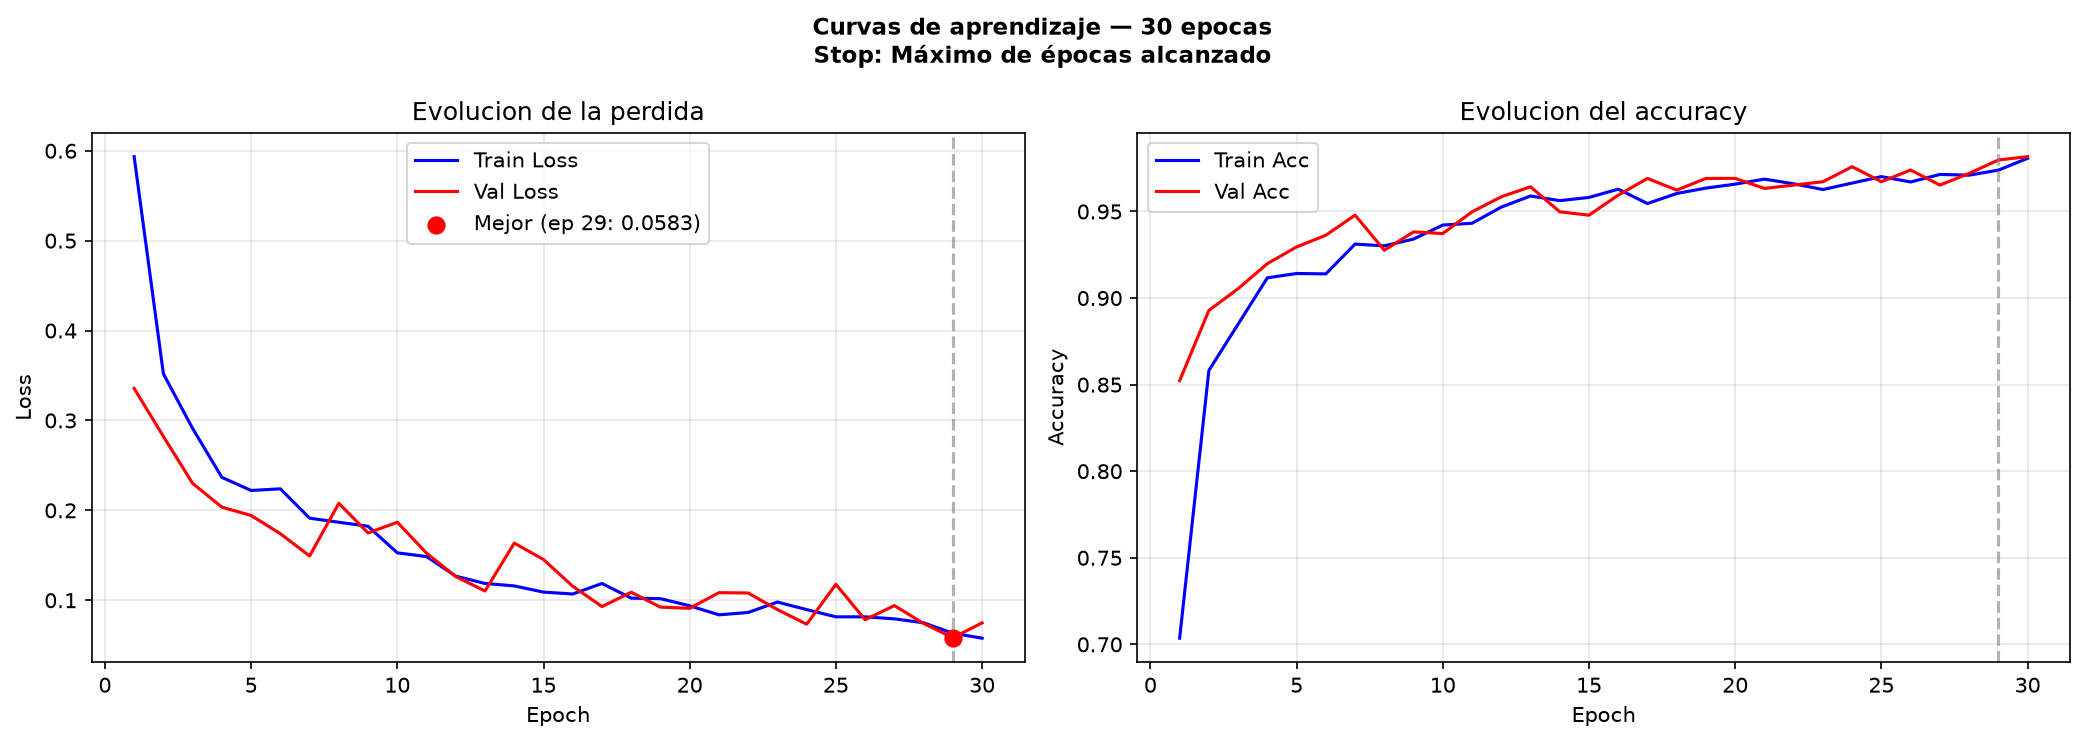
\includegraphics[width=0.95\columnwidth]{../BrainTumor/results/swin/normalized_scratch/learning_curves.png}
    \caption{Curvas de aprendizaje de Swin-T desde cero con pipeline normalizado.}
    \label{fig:swin_scratch_lc}
\end{figure}
